
%
% File: chap03.tex
% Author: Antigoni Kourou
% Description: The proposed approach
%
\let\textcircled=\pgftextcircled
\chapter{The proposed approach}

\label{chap:prop}

\initial{F}or estimating a discrete score of opinion on every accommodation feature mentioned in the text feedback of a listing, this paper proposes an approach as shown in Figure \ref{fig:pipe}. The pipeline consists of four main steps: \textit{pre-processing, feature identification, sentiment detection}  and \textit{data analysis}. Initially, the whole corpus of text data is pre-processed as it will be described in the following section. Features and sentiment are then identified in text based in sentence level. The output of the three first stages is re-organized and analyzed to match different customer needs. 
The whole pipeline is built using Python programming language and its related packages. The following sections will explain each step of the proposed approach in further details.
\section{Pre-processing}
The algorithm deals with a huge set of reviews, which are retrieved from the feedback system of Airbnb and they serve as the input of the pipeline. The whole corpus of reviews consists of 3.4GB, including reviews of the listings from the Netherlands, which is filtered to be focused only in Amsterdam. The data set is stored in cloud, in the Neo4J graph database, where the nodes can represent a listing, a guest or host, review or response. (Appendix figure?)
Python is connected to read the data from cloud, using Cypher querying language for Neo4J. The reviews in the set are read one by one and each of them is checked if it fulfills the language requirements. In my work, the whole concept of the pipeline is developed in English, as the most used language, therefore every time that the algorithm runs into a review not in English, it will ignore the review and continue with the next one. For the English reviews, the algorithm will split the text into sentences, 
\begin{figure}[h!]
	\centering
	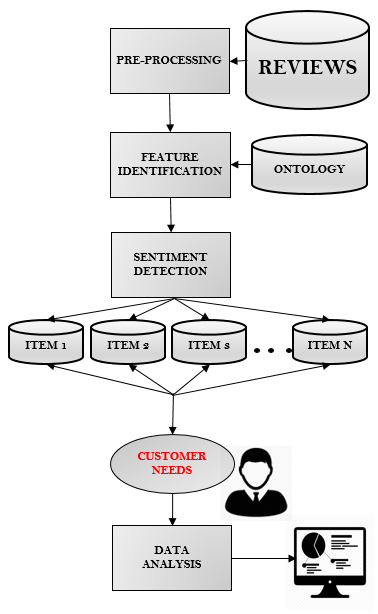
\includegraphics[height=0.72\textheight]{Pipeline1}
	\caption{The proposed approach}
	\label{fig:pipe}
\end{figure} 
thus the sentiment detector would refer to each sentence within the review.
%
After having created a nested-list consisting of reviews and their sentences, tokenization and lemmatizing are performed on in order to cut each sentence into words, which are candidates for representing an accommodation feature. For tokenization the pipeline uses the TweetTokenizer\footnote{http://www.nltk.org/api/nltk.tokenize.html} package, part of NLTK and Twitter-aware designed, in order to be able to identify emoticons and adapt to new domains. On the other hand lemmatization is achieved using WordNet library. The output of these two steps is a list of lemmas for each sentence. 

\section{Feature identification}

As soon as each sentence in the corpus of reviews is represented as a list of lemmas, an ontology based approach is used to identify the accommodation features of each sentence. The ontology is chosen for feature identification as a way for detecting all the terms, concepts and relations linked to accommodation domain.Prior to identifying the features, the pipeline builds a list of synonyms, hyponyms and hypernyms for every term of the ontology. The list is based on the Synsets and relations between concepts as introduced by WordNet library. The lists of related terms is lemmatized and the duplicates are removed. The lemmatization process aims to create a list of related lemmas for each feature in the ontology, which would then be used for feature identification in the sentences.
Thus, the feature identification steps is a string match of the list of lemmas for every single sentence, with the list of related lemmas of every feature in the ontology. Considering that the ontology consists of many terms, this sample pipeline is trained with 6 features, namely \textit{accuracy, cleanliness, check-in, communication, location} and \textit{value}. These features are chosen based on the features that Airbnb asks the users to manually rate as part of their feedback.

\section{Sentiment detection}
After pre-processing and feature identification, a very important part of the pipeline is sentiment detection. The algorithm used for this purpose is VADER \footnote{https://pypi.python.org/pypi/vaderSentiment}, part of Python packages. VADER is a lexicon and rule-based sentiment analysis tool that is specifically attuned to sentiments expressed in social media. Based on the comparisons of 22 sentiment mining tools on specific contexts, VADER is ranked as the best algorithm for comments and the second best for social networks \cite{ribeiro2015benchmark}.
VADER is able to deal with negation, capital letters, emoticons, punctuation types, \textit{but} sentences and slangs. The pipeline asks uses VADER to return a sentiment score for every sentence of the review, which would afterwards be a score for the identified features in that sentence. Considering that in one sentence, more than 1 feature can be identified, a probabilistic model is used for defining the probabilities that a sentiment score would reflect user's opinion for the features identified within one sentence. For a better understanding, let's have a look at the whole model of data, including the probabilistic sentiment scores.

The whole data corpus consists of 11 053 listings. Each listing in this corpus can be represented by the ID of the listing in the database L\textsubscript{lis\_id}. Every listing from this set has a number of reviews, which varies from one listing to the other and is identified from ID of the review \textit{R\textsubscript{lis\_id} = \{ R\textsubscript{0}, R\textsubscript{1},  R\textsubscript{2} ... R\textsubscript{r} \}}. For a single review of a certain listing would be \textit{R\textsubscript{lis\_id, rev\_id}}. This review is composed by a number of sentences \textit{S\textsubscript{lis\_id, rev\_id} = \{S\textsubscript{0}, S\textsubscript{1}, S\textsubscript{2} ... S\textsubscript{s}\}}. 
The pipeline is trained to detect the sentiment of all the sentences, which will be in the same form as the one above. 
In each of these sentences, the pipeline is trained to identify six accommodation features \textit{F = \{accuracy, check-in, cleanliness, communication, location, value\}}. When the sentiment of a sentence is detected, it does not particularly refer to a certain feature. In order to calculate the part of the sentiment that belongs to a certain feature identified in the sentence, we use a probabilistic model. According to this model, the probability that the compound sentiment score refers to a certain feature is p\textsubscript{i}, where \textit{i} is the index of the feature from the list F. This probability is uniformly distributed between the identified features and is calculated as 1/k, where \textit{k} is the number of features mentioned. Likewise, if the feature is not identified in the sentence the probability would be 0.
%
% ----------------FORMULA---------------------
$$Sentiment = \sum_{i=1}^{n}p\textsubscript{i} *  sentiment\textsubscript{ i}$$ 
%---------------------------------------------
%
This formula for calculating the sentiment of the features is part of the sentiment detection phase of the pipeline and it is repeated for every single sentence. For instance, considering the reviews of listing 24328,  \textit{R\textsubscript{24328, 10146}} would represent the review: "We had a great stay at Joe's. The handy guide to the house and neighborhood was much appreciated, as were Joe's clear instructions for checking in while he was away. The house was comfortable and eclectic, full of personal character." Thus, \textit{S\textsubscript{24328, 10146, 1}} represents the second sentence of the text above. In this sentence can be identified three features \textit{check-in, communication,} and \textit{location}. The compound sentiment score of the sentence above has in this way to refer to one of these features in a probability of 33.3\%. Figure \ref{fig:sent} shows the results of the pipeline for this case. The output of the whole sentiment detection phase is a Comma Separated Vector (.csv) file, consisting of all listings, all listings' reviews, its respective sentences and the sentiment for the identified features on these sentences. 
\begin{figure}[h!]
	\centering
	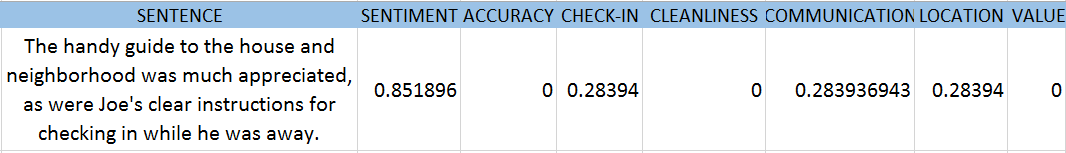
\includegraphics[height=0.1\textheight]{example_pip}
	\caption{Example of the probabilistic sentiment results}
	\label{fig:sent}
\end{figure}
%

\section{Data analysis}

% 
% will explain the analysis process using Pandas for different cases! 
%
